\section{Installing Standard Programs:}

\subsection{Installing {\tt HepMC}}
{\tt
wget -c '\url{http://lcgapp.cern.ch/project/simu/HepMC/download/HepMC-2.06.09.tar.gz}'\\
tar -xf 'HepMC-2.06.09.tar.gz'\\
cd 'HepMC-2.06.09/'\\
'./configure' '--with-momentum=GEV' '--with-length=MM'\\
make -j4\\
sudo make install\\
}

\subsection{Installing {\tt FastJet}:}
{\tt
wget -c '\url{http://www.fastjet.fr/repo/fastjet-3.3.0.tar.gz}'\\
tar -xf './fastjet-3.3.0.tar.gz'\\
cd fastjet-3.3.0/\\
./configure\\
make -j4\\
sudo make install\\
}

\subsection{Installing {\tt Pythia8}:}
{\tt
wget -c '\url{http://home.thep.lu.se/~torbjorn/pythia8/pythia8230.tgz}'\\
tar -xf 'pythia8230.tgz'\\
cd 'pythia8230/'\\
./configure '--with-hepmc2'\\
make -j4\\
sudo make install\\
}

\subsection{Installing {\tt Root-6}}
Download the binary distribution from \url{https://root.cern.ch/content/release-61206} for the appropriate platform and extract.
Once you have extracted, you will get a directory "root" wherever you extracted, cd to this directory and run
{\tt source root/bin/thisroot.sh} (assuming you are using bash shell, otherwise modify accordingly). If you are installing {\tt root} to a non standard directory, it is preferable to put "source root/bin/thisroot.sh" into your {\tt "~/.bashrc"} (or some other initialization file for your shell).

If this method does not produce a good executable then you should compile root from source, please follow the instructions from the official (\url{https://root.cern.ch/building-root}) site (please do not use non-standard scripts / commands from random forums).

\subsection{Installing {\tt Delphes}}
{\tt
	wget -c '\url{http://cp3.irmp.ucl.ac.be/downloads/Delphes-3.4.1.tar.gz}'\\
	tar -xf './Delphes-3.4.1.tar.gz'\\
	cd './Delphes-3.4.1/'\\
	'./configure'\\
	make -j4\\	
}\\
Delphes does not have any "make install" but all the executables you need are produced in the source directory and can be copied anywhere required.
An important step required is to manually copy "libDelphes.so" to '/usr/local/lib' or any other library search path and also copy all the root dictionaries
({\tt 'ClassesDict\_rdict.pcm', 'ExRootAnalysisDict\_rdict.pcm', 'FastJetDict\_rdict.pcm',\\ 'ModulesDict\_rdict.pcm'}) to the root dictionary search path and copy the header files ({\tt 'classes', 'external'} folders) to the default headers search paths ({\tt '/usr/local/include'}).

\section{Generating the events:}
The event generation is done in {\pyth} and written in {\tt HepMC} formate.
The example program {\tt main41.cc} inside pythia examples folder contains a sample program to generate events using {\pyth} and write to {\tt HepMC} formate.
{\tt HepMC} files produced tend to be very big so its recommended to not store them on disk instead just generate them and use them in {\tt Delphes} on the fly, this is done using \href{http://man7.org/linux/man-pages/man7/fifo.7.html}{fifo}.
The complete arrangement can be found in the {\tt Generator} class of {\tt all.cc} (this also requires {\tt Delphes} to be installed and in the accessible in the folders listed in {\tt PATH} variable of the shell). {\tt Delphes} also requires the detector model to simulate, we are using  {\tt delphes\_card\_CMS.tcl} (this does not simulate any pile-up).

\section{Results:}

A simple starting point for tagging might be:\\
(\href{https://arxiv.org/pdf/0802.2470.pdf}{arXiv:0802.2470 [hep-ph]}) {\bf Jonathan M. Butterworth, Adam R. Davison, Mathieu Rubin, Gavin P. Salam:} Jet substructure as a new Higgs search channel at the LHC.\\
This method is incorporated in the class {\tt NewHEPHeaders::MassDropTagger::HardSubStructureFinder} of the file {\tt NewHEPHeaders4.hh}

\begin{figure}
	\begin{center}
		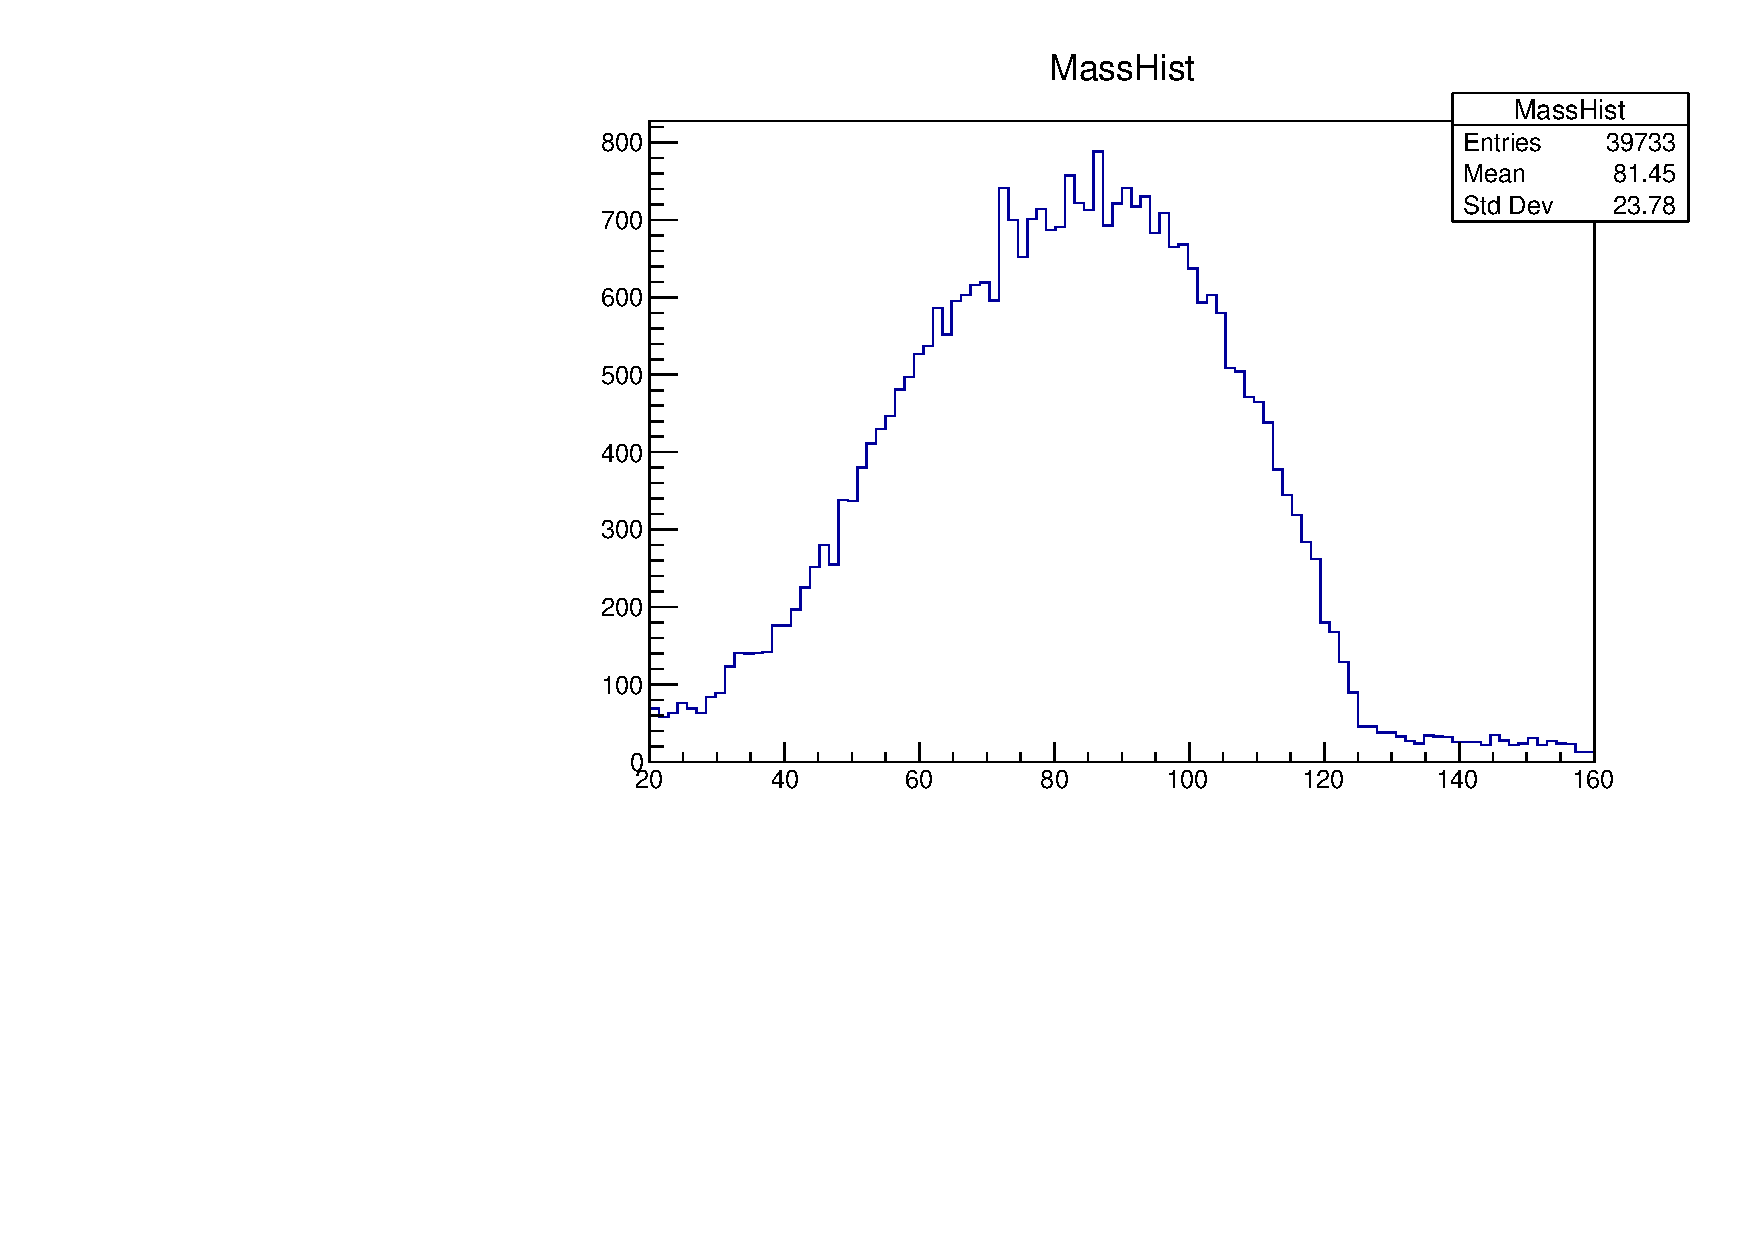
\includegraphics[width=0.9\textwidth]{MassDropTaggerResult.pdf}
		\caption{
			The invariant mass of the leading (by $p_T$) fat jet ($R=1.0$, $p_T^{j}>100$ GeV) after applying the mass drop check (for 2 prong) and filtering on the fat jet. Generator level vectors are used here without any {\tt Delphes} effects.
		}
	\end{center}
\end{figure}

\begin{figure}
	\begin{center}
		\includegraphics[width=0.9\textwidth]{MassHistTowers.pdf}
		\caption{
			The invariant mass of the leading (by $p_T$) fat jet ($R=1.0$, $p_T^{j}>100$ GeV) after applying the mass drop check (for 2 prong) and filtering on the fat jet. Calorimeter tower vectors are used here.
		}
	\end{center}
\end{figure}

\begin{figure}
	\begin{center}
		\includegraphics[width=0.9\textwidth]{MassHistEFlow.pdf}
		\caption{
			The invariant mass of the leading (by $p_T$) fat jet ($R=1.0$, $p_T^{j}>100$ GeV) after applying the mass drop check (for 2 prong) and filtering on the fat jet. EFlow vectors are used here.
		}
	\end{center}
\end{figure}